\osoba{Adam Walczak}
\zadanieprojektowe{W  jaki sposób nasz smartfon może być lokalizowany i do czego to służy}{2015-10-29}{2015-10-31}{zakończone}
Najbardziej dokładnym, a co za tym idzie najważniejszym sposobem na lokalizację jest system GPS. Jest to system nawigacji satelitarnej używany do precyzyjnego pozycjonowanie urządzeń lub namierzania celów.
do zastosowań cywilnych dokładność pomiarów jest ustalona na poziomie 1-3 m. W praktyce sami możemy to określić. Wskazania rzeczywiście mogą pokazywać waszą dokładną pozycję lub oddaloną nawet o 20-30 metrów. Uśredniając możecie zlokalizować smartfona z dokładnością 4-12 m. Wszystko zależy od ilości widocznych satelitów, ukształtowania terenu, warunków atmosferycznych oraz naturalnych przeszkód.
\begin{figure}[H]
\centering
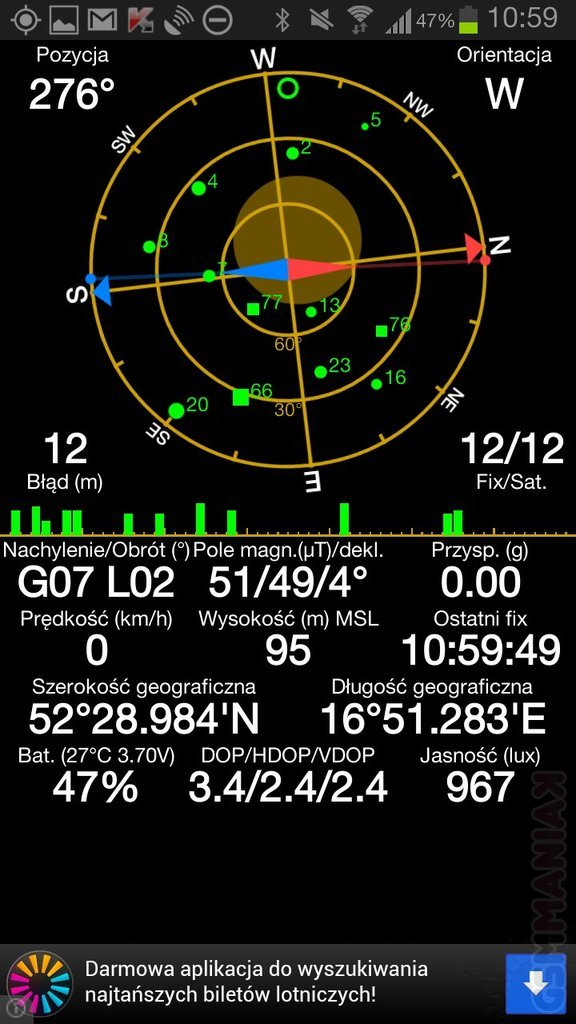
\includegraphics[scale=0.25]{czlonkowie/5/1ss.jpg}
\end{figure}
Prawdą jest, że odbiornik, który posiadamy w smartfonach to tak na prawdę A-GPS. Przedrostek “A” oznacza, że jest to system wspomagany przez sieć komórkową. Największym problemem jest prędkość znalezienia sygnału. Odbiorniki w smartfonach są małe, a w dodatku często używane w miastach gdzie są wysokie budynki, które nie pomagają w lokalizacji. Transmisja danych pozwala na pobranie danych, które dostarczają informacji modułowi GPS, w której części nieboskłonu ma szukać satelitów. W momencie kiedy połączenie z pierwszym zostanie ustanowione na podstawie porównań odbiornik znajdzie już pozostałe. Transmisja danych znacząco przyśpiesza połączenie z satelitami. Różnica między ustanowieniem lokalizacji bez transmisji danych, a z włączonym Internetem może wynosić 5-10 sekund do 3-5 minut. W najnowszych smartfonach jest już stosowany system Glonass. Jest to rosyjski odpowiednik GPS (amerykański). Korzystanie z dwóch odbiorników naraz poprawia dokładność i przyśpiesza wskazanie naszego położenia.
\begin{figure}[H]
\centering
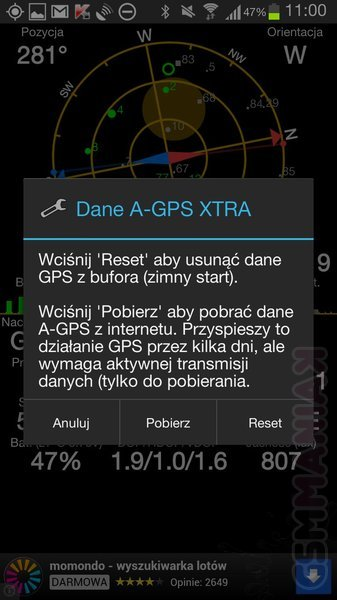
\includegraphics[scale=0.5]{czlonkowie/5/2ss.jpg}
\end{figure}
Drugim sposobem na lokalizację jest użycie sieci bezprzewodowej WiFi. Najważniejszym faktem jest, że nie musimy być połączeni z samą siecią, żeby udostępnić smartfonowi swoją pozycję. Skanuje on pobliskie sieci i na podstawie mocy sygnału (odległość od routera) określa nasze położenie. Ten typ lokalizacji nie jest dokładny ale przydaje się strasznie w budynkach, kiedy sygnał GPS lub Glonass jest niski lub nie ma go wcale. W praktyce dokładność lokalizacji jest na poziomie 200 m i większa. Wszystko zależy od ilości sieci WiFi w naszym otoczeniu.
\begin{figure}[H]
\centering
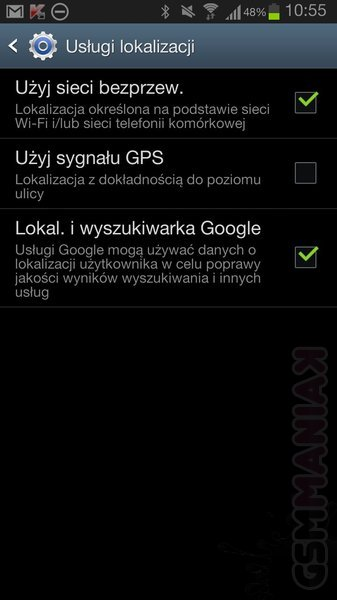
\includegraphics[scale=0.5]{czlonkowie/5/3ss.jpg}
\end{figure}
Trzecim sposobem jest lokalizacja na podstawie stacji bazowych sieci komórkowych tzw.BTS. Tu dokładność jest najmniejsza. Maszty operatorów mogą być oddalone od siebie nawet o kilka kilometrów. Zapewne pamiętacie w starych nokiach takie rozwiązania jak pokazywanie ulicy pod nazwą operatora. Jest to nadal realizowane właśnie na podstawie BTSów, które przesyłają dane do naszego smartfona. Cały szereg urządzeń takich jak akcelerometr, kompas, żyroskop czy barometr pomagają poprawić dokładność lokalizacji. Wspomagają one nawigację w ruchu. Ich użycie również wpływa na zmniejszenie zużycia energii w smartfonie poprzez ograniczenie korzystania z odbiornika GPS czy WiFi
\begin{figure}[H]
\centering
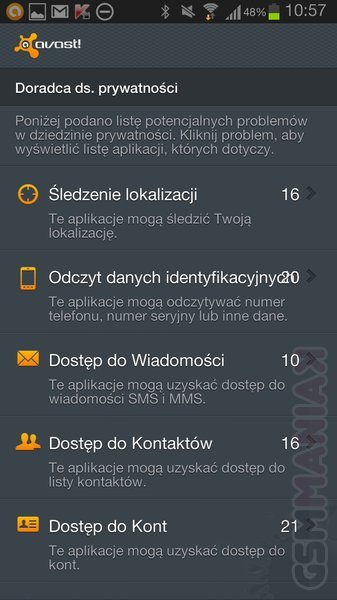
\includegraphics[scale=0.5]{czlonkowie/5/4ss.jpg}
\end{figure}
Liczba aplikacji, która korzysta z dostępu do lokalizacji jest ogromna. Czasami nawet możecie nie zdawać sobie z tego sprawy. Od taki program do korzystania z usług bankowych. Pozwala na sprawdzanie stanu konta, robienie przelewów czy przeglądanie historii. Jeśli nikt nie wchodził w dodatkowe opcje może się zdziwić skąd w wymaganych uprawnieniach tej aplikacji dostęp do lokalizacji. Na podstawie tych danych program jest wstanie wskazać nam najbliższe placówki banku oraz bankomaty. Zastanawiacie się pewnie czy to jest bezpieczne? Postanowiłem sobie zostawić ten temat na sam koniec.
\begin{figure}[H]
\centering

\includegraphics[scale=0.5]{czlonkowie/5/5ss.jpg}
\end{figure}
Ustawienia lokalizacji czy współrzędnych w Mapach Google są bardzo przydatnymi funkcjami. Dzięki nim nasi znajomi są nieustannie informowani gdzie się znajdujemy. Możemy w łatwy sposób znaleźć drogę do szukanego przez nas miejsca czy zlokalizować punkt użyteczności publicznej. Miejmy na uwadze, że ciągłe korzystanie z GPS oraz dzielenie się pozycją znacząco podnosi zużycie energii w smartfonie.
\begin{figure}[H]
\centering
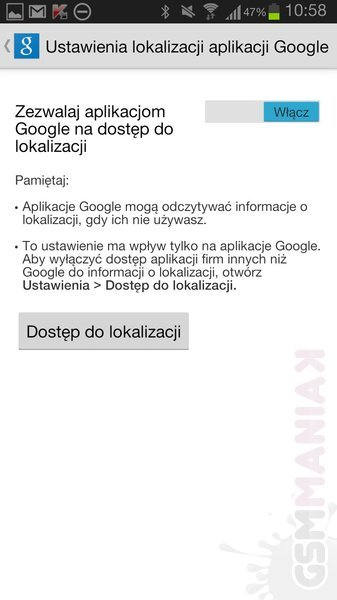
\includegraphics[scale=0.5]{czlonkowie/5/6ss.jpg}
\end{figure}

\zadanieprojektowe{Czynniki wpływające na wynik pomiaru GPS, wady i zalety GPS}{2015-11-06}{2015-11-08}{zakończone}

Czynniki wpływające na wynik pomiaru GPS : \newline

******Satelity******
>>   Parametry orbity - dokładność wyznaczenia położenia
>>   środek fazowy anteny na satelicie
>>   pole grawitacyjne Ziemi
>>   opór atmosfery
>>   przyciąganie grawitacyjne ciał niebieskich (m.in. Słońca i Księżyca)
>>   oddziaływanie sił elektromagnetycznych
>>   ciśnienie światła słonecznego
>>   efekty relatywistyczne
     <>  OTW - ruch zegara w polu grawitacyjnym (zegar przyśpiesza o około 45.9 ns/doba)
     <>  STW - ruch zegara (zegar zwalnia około -7.2ns/doba)\newline

******Odbiorniki******
>>   niestabilność wzorców częstotliwości
>>   poprawki zegarów odbiorników
>>   cycle slip - nieciągłość fazy, czyli zmiana skokowa rejestrowanej fazy
>>   nieoznaczoność fazy
>>   środki fazowe anten odbiorników
>>   szum odbiornika
>>   rodzaj obserwacji - statyczne, kinematyczne, PPP
>>   odzyskiwanie fali nośnej L2 - dla pomiarów precyzyjnych\newline

******Zakłócenia propagacyjne******
>>   refrakcja troposfery i opóźnienie troposferyczne
>>   refrakcja jonosfery
>>   szumy atmosferyczne i kosmiczne
>>   odbicia i interferencja fal wtórnych\newline

******Zjawiska geofizyczne******
>>   nutacja
>>   ruch biegunów
>>   pływy skorupy ziemskiej
>>   pływy oceaniczne
>>   ruchy płyt tektonicznych
>>   oceaniczny efekt obciążeniowy\newline

******Pozostałe******
>>   nieciągłości fazy
>>   różnica czasu pomiędzy UT1 i UTC
>>   parametry transformacji między układami współrzędnych
>>   anti-spoofing (zapobieganie intencjonalnym próbom zakłócenia pracy systemu poprzez zmianę kodu P na Y)
>>   selective availability - zakłócanie sygnału cywilnego (czas i parametry satelity) pseudolosowym błędem - obecnie wyłączone\newline


Wady i zalety GPS \newline

Zalety:\newline

1.  Pomiary GPS są w zasadzie niezależne od warunków meteorologicznych na stanowiskach obserwacyjnych.\newline 


2.  Techniki obserwacyjne GPS nie wymagają wzajemnej widoczności obserwowanych punktów; wymagają natomiast odkrytego nieboskłonu od wysokości 150 od horyzontu. Nie jest zatem wymagana budowa specjalnych wież i stanowisk podwyższonych, jak to miało miejsce przy stosowaniu klasycznych technik naziemnych. Punkty sieci GPS można i należy lokalizować nie na trudno dostępnych wzgórzach, lecz w łatwo dostępnych miejscach przy szlakach komunikacyjnych. \newline \newline


3.  Pomiar satelitarny na stanowisku trwa bardzo krótko (pomiar statyczny dla punktów o znaczeniu lokalnym trwa około 45-60 minut, pomiar technologią szybką statyczną - 15-20 minut, zaś technologią "stop and go" tylko 1-2 minuty); dla niektórych prac geodezyjnych można stosować pomiary w czasie rzeczywistym (real time kinematic) dające wyniki natychmiast w terenie.\newline


4.  Dokładność pomiarów GPS jest na ogół wyższa od dokładności klasycznych metod obserwacyjnych. Przypomnijmy, że standardowa dokładność statycznych pomiarów względnych GPS wynosi 10-6.\newline


5.  Pomiar GPS na stanowisku jest w pełni zautomatyzowany. Wstępne opracowanie danych polowych może być opracowane od razu w terenie. Przy odpowiednio przygotowanym i realizowanym harmonogramie prac terenowych pełne opracowanie sieci może być prowadzone sukcesywnie.\newline


6.  Wyniki pomiarów GPS uzyskuje się w jednolitym geocentrycznym układzie współrzędnych globalnych. Poprzez nawiązanie pomiarów satelitarnych do istniejących punktów sieci krajowych uzyskuje się możliwość obliczenia parametrów transformacyjnych i współrzędnych wszystkich wyznaczanych punktów w układzie współrzędnych obowiązujących w danym kraju. Takie parametry transformacji są już wyznaczone dla układów współrzędnych obowiązujących w Polsce.\newline


7.  Wyznaczanie położenia punktów sieci metodami satelitarnymi GPS jest niezależne; nie występuje tu znane w klasycznej geodezji prawo przenoszenia się błędów w sieciach geodezyjnych.\newline


8.  Pomiary różnicowe GPS dostarczają jakościowo nowych elementów sieci, którymi są różnice współrzędnych X, Y, Z. Pomiary te dają zatem możność wyznaczenia zarówno skali jak i orientacji sieci.\newline


9.  Technologie pomiarów GPS są wysoce ekonomiczne. Koszt aparatury zwraca się bardzo szybko. Warto pamiętać, że koszt jednego odbiornika GPS wynosi tyle, ile kosztuje budowa 8-9 kilkunastometrowej wysokości wież triangulacyjnych.\newline

Wady:\newline

1.  Celowo wprowadzona degradacja sygnałów satelitów GPS powoduje znaczne zmniejszenie dokładności pomiarów bezwzględnych, a także różnicowych (względnych) w tych przypadkach, gdy użytkownik nie dysponuje odpowiednio zaawansowanymi odbiornikami, które mogą wyeliminować wpływ degradacji "anti-spoofing".\newline


2.  Niektóre technologie GPS wymagają nieprzerwanej łączności z satelitami podczas całej sesji pomiarowej (np. technologia "stop and 
go").\newline


3.  Występujące niekiedy zakłócenia w odbiorze sygnałów satelitarnych powodują przerwy w ciągłości pomiaru i tzw. utratę cykli. Fakt ten utrudnia opracowanie i wymaga dokonania najpierw rekonstrukcji cykli.\newline


4.  Satelity GPS dokonują dwóch obiegów wokół Ziemi w ciągu jednej doby. Powoduje to, że każdego dnia w określonym momencie czasu pojawia się taka sama konfiguracja satelitów GPS; pomiary wykonywane w tej samej porze dnia obarczone są zatem błędem konfiguracji geometrycznej konstelacji satelitów GPS.\newline